\documentclass{article}
\usepackage{amsmath, sfmath, multicol, tkz-euclide, array, enumerate, tcolorbox, tabularray}
\renewcommand{\familydefault}{\sfdefault}
\setlength{\parindent}{0cm}
\pagestyle{empty}
\usepackage[left=1in, top=0.5in, right=1in, bottom=0.5in]{geometry}
\tcbset{colback=white}

\newcounter{example}[section]
\newenvironment{example}[1][]{\refstepcounter{example}\par\medskip
   {\color{red}\textbf{Example~\theexample. #1}}}{\medskip}

\begin{document}

\section*{Measuring Segments}

\begin{tcolorbox}[colframe=orange!70!white, coltitle=black, title=\textbf{Today I Can}]
\begin{enumerate}
    \item Find and compare the lengths of segments.
\end{enumerate}
\end{tcolorbox}

\subsection*{Distance on a Number Line}

To find the distance between two points $A$ and $B$ on a number line, subtract their coordinates and take the absolute value.
\[
|A - B|
\]

\begin{example}
Given the number line below, find each distance.

\begin{center}
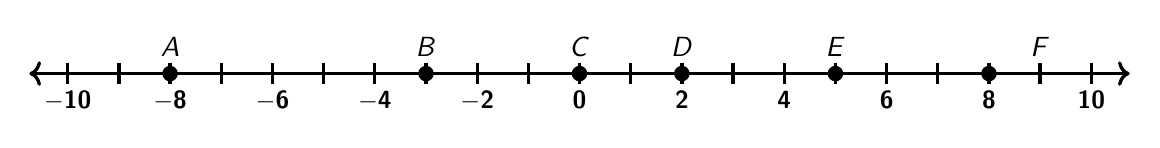
\begin{tikzpicture}[scale = 0.65]
    \foreach \x in {-10, -9, ..., -1, 0, 1, 2, ..., 10}
    \draw[very thick] (\x, 0.2) -- (\x, -0.2);
    \foreach \x in {-10, -8, -6, -4, -2, 0, 2, 4, 6, 8, 10}
    \node at (\x, -0.15) [below] {\small $\mathbf{\x}$};
    \draw[very thick, <->] (-10.75, 0) -- (10.75, 0);
    \draw [fill=black] (-8,0) circle (4pt);
    \node at (-8,0.15) [anchor = south] {$A$};
    \draw [fill=black] (-3,0) circle (4pt);
    \node at (-3,0.15) [anchor = south] {$B$};
    \draw [fill=black] (0,0) circle (4pt);
    \node at (0,0.15) [anchor = south] {$C$};
    \draw [fill=black] (2,0) circle (4pt);
    \node at (2,0.15) [anchor = south] {$D$};
    \draw [fill=black] (5,0) circle (4pt);
    \node at (5,0.15) [anchor = south] {$E$};
    \draw [fill=black] (8,0) circle (4pt);
    \node at (9,0.15) [anchor = south] {$F$};
\end{tikzpicture}
\vspace{0.2in}
\end{center}

\begin{multicols}{3}
\begin{enumerate}[(a)]
    \item $AC$
    \item $BE$
    \item $CF$
\end{enumerate}
\end{multicols}
\end{example}
\vspace{0.25in}

\subsection*{Segment Addition Postulate}

\begin{tcolorbox}[
colframe=black!20!white, 
opacitybacktitle=0.1,
coltitle=black, title=\textbf{Segment Addition Postulate}]
If 3 points $A$, $B$, and $C$ are collinear and $B$ is between $A$ and $C$, then $AB + BC = AC$.
\begin{center}
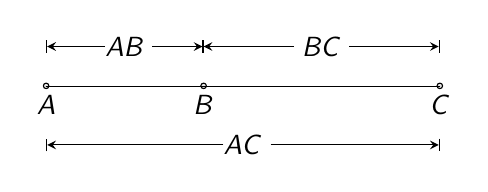
\begin{tikzpicture}
\tkzDefPoints{0/0/A, 2/0/B, 5/0/C}
\tkzDrawPoints(A,B,C)
\tkzLabelPoints[below](A,B,C)
\tkzDrawSegment(A,C)
\node at (1,0.5) {$AB$};
\node at (3.5,0.5) {$BC$};
\node at (2.5,-0.75) {$AC$};
\draw [->|, >=stealth](0.75,0.5) -- (0,0.5);
\draw [->|, >=stealth](1.35,0.5) -- (2,0.5);
\draw [->, >=stealth](3.15,0.5) -- (2,0.5);
\draw [->|, >=stealth](3.85,0.5) -- (5,0.5);
\draw [->|, >=stealth](2.25,-0.75) -- (0,-0.75);
\draw [->|, >=stealth](2.85,-0.75) -- (5,-0.75);
\end{tikzpicture}
\end{center}
\end{tcolorbox}
\vspace{0.25in}

\begin{example}
If $EG=59$, what are $EF$ and $FG$?
\bigskip 

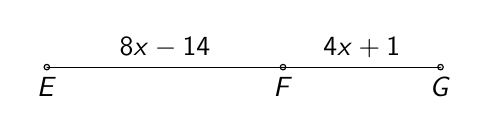
\begin{tikzpicture}
    \tkzDefPoints{0/0/E, 3/0/F, 5/0/G}
    \tkzDrawPoints(E,F,G)
    \tkzLabelPoints[below](E,F,G)
    \tkzDrawSegment(E,G)
    \tkzLabelSegment[above](E,F){$8x-14$}
    \tkzLabelSegment[above](F,G){$4x+1$}
\end{tikzpicture}
\end{example}
\vfill 

\begin{example}
If $JL=120$, what are $JK$ and $KL$?
\bigskip 

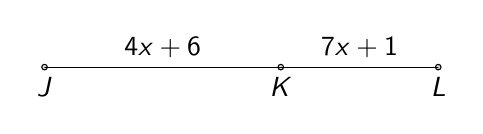
\begin{tikzpicture}
    \tkzDefPoints{0/0/J, 3/0/K, 5/0/L}
    \tkzDrawPoints(J,K,L)
    \tkzLabelPoints[below](J,K,L)
    \tkzDrawSegment(J,L)
    \tkzLabelSegment[above](J,K){$4x+6$}
    \tkzLabelSegment[above](K,L){$7x+1$}
\end{tikzpicture}
\end{example}
\vfill 

\newpage 

\begin{tcolorbox}[
colframe=black!20!white, 
opacitybacktitle=0.1,
coltitle=black, title=\textbf{Congruent}]
Equal in measure
\end{tcolorbox}

Segments that have the same length are \textbf{congruent}. The symbol for congruent is $\cong$.
\newline\\

\begin{tikzpicture}
    \tkzDefPoints{0/0/A, 2.5/0/B, 0/-2/C, 2.5/-2/D}
    \tkzDrawPoints(A,B,C,D)
    \tkzLabelPoints[below](A,B,C,D)
    \tkzDrawSegments(A,B C,D)
    \tkzLabelSegment[above](A,B){1 in.}
    \tkzLabelSegment[above](C,D){1 in.}
    \node at (1.25,-3.5) {$AB = CD$};
    \node at (4,0) {$\longrightarrow$};
    \node at (4,-2) {$\longrightarrow$};
\end{tikzpicture}
\hspace{0.15in}
\begin{tikzpicture}
    \tkzDefPoints{0/0/A, 2.5/0/B, 0/-2/C, 2.5/-2/D}
    \tkzDrawPoints(A,B,C,D)
    \tkzLabelPoints[below](A,B,C,D)
    \tkzDrawSegments(A,B C,D)
    \tkzMarkSegments[mark=|](A,B C,D)
    \node at (1.25,-3.5) {$AB \cong CD$};
\end{tikzpicture}

\bigskip 

\begin{example}
Are $\overline{AC}$ and $\overline{BE}$ congruent?\newline\\

\begin{center}
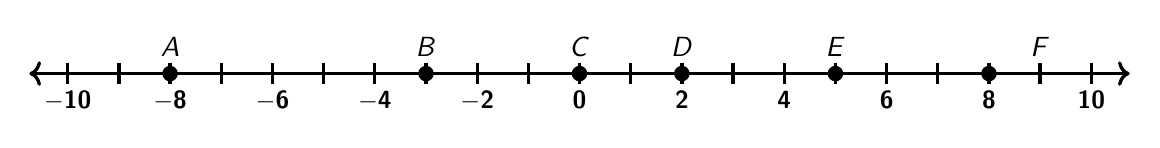
\begin{tikzpicture}[scale = 0.65]
    \foreach \x in {-10, -9, ..., -1, 0, 1, 2, ..., 10}
    \draw[very thick] (\x, 0.2) -- (\x, -0.2);
    \foreach \x in {-10, -8, -6, -4, -2, 0, 2, 4, 6, 8, 10}
    \node at (\x, -0.15) [below] {\small $\mathbf{\x}$};
    \draw[very thick, <->] (-10.75, 0) -- (10.75, 0);
    \draw [fill=black] (-8,0) circle (4pt);
    \node at (-8,0.15) [anchor = south] {$A$};
    \draw [fill=black] (-3,0) circle (4pt);
    \node at (-3,0.15) [anchor = south] {$B$};
    \draw [fill=black] (0,0) circle (4pt);
    \node at (0,0.15) [anchor = south] {$C$};
    \draw [fill=black] (2,0) circle (4pt);
    \node at (2,0.15) [anchor = south] {$D$};
    \draw [fill=black] (5,0) circle (4pt);
    \node at (5,0.15) [anchor = south] {$E$};
    \draw [fill=black] (8,0) circle (4pt);
    \node at (9,0.15) [anchor = south] {$F$};
\end{tikzpicture}
\end{center}
\end{example}

\vspace{0.25in}

\begin{tcolorbox}[
colframe=black!20!white, 
opacitybacktitle=0.1,
coltitle=black, title=\textbf{Midpoint}]
A point that divides a segment into 2 congruent segments. In the picture below, $B$ is the midpoint of $\overline{AC}$.

\begin{center}
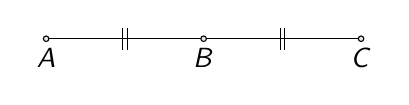
\begin{tikzpicture}
    \tkzDefPoints{0/0/A, 2/0/B, 4/0/C}
    \tkzDrawSegment(A,C)
    \tkzDrawPoints(A,B,C)
    \tkzLabelPoints[below](A,B,C)
    \tkzMarkSegments[mark = ||](A,B B,C)
\end{tikzpicture}
\end{center}
\end{tcolorbox}

\vspace{0.2in}

\begin{example}
$Q$ is the midpoint of $PR$. What are $PQ$, $QR$, and $PR$?
\bigskip 

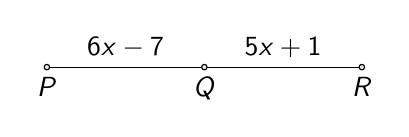
\begin{tikzpicture}
    \tkzDefPoints{0/0/P, 2/0/Q, 4/0/R}
    \tkzDrawSegments(P,Q Q,R)
    \tkzDrawPoints(P,Q,R)
    \tkzLabelPoints[below](P,Q,R)
    \tkzLabelSegment[above](P,Q){$6x-7$}
    \tkzLabelSegment[above](R,Q){$5x+1$}
\end{tikzpicture}
\end{example}

\vfill 

\begin{example}
$U$ is the midpoint of $TV$. What are $TU$, $UV$, and $TV$?
\bigskip 

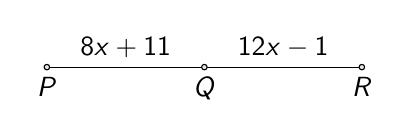
\begin{tikzpicture}
    \tkzDefPoints{0/0/P, 2/0/Q, 4/0/R}
    \tkzDrawSegments(P,Q Q,R)
    \tkzDrawPoints(P,Q,R)
    \tkzLabelPoints[below](P,Q,R)
    \tkzLabelSegment[above](P,Q){$8x+11$}
    \tkzLabelSegment[above](R,Q){$12x-1$}
\end{tikzpicture}
\end{example} 

\vfill 

\end{document}
